


%----------------------------------------------------------------------------------------

\newpage

%\chapter{Thematic Developments}{Développements Thématiques} % Chapter title
\chapter{Développements thématiques}

\markboth{\thechapter\space Développements Thématiques}{\thechapter\space Développements Thématiques}

\label{app:thematic} % For referencing the chapter elsewhere, use \autoref{ch:name} 

%----------------------------------------------------------------------------------------


Cette annexe regroupe des développements thématiques, c'est à dire qui tombent dans les domaines empiriques, conceptuels et de modélisation. Elles peuvent être relativement éloignées à première vue de nos préoccupations principales, mais sont nécessaires pour la démonstration de points précis.


Les trois premiers développements sont importants quant à des questions empiriques, de modélisation et de méthodologie, abordées d'un point de vue thématique précis.
\begin{enumerate}
	\item Une étude empirique de la géographie des prix du carburant aux Etats-unis, permet, sous l'hypothèse que celle-ci capture des processus à l'interface du réseau routier et des territoires, de mettre en valeur deux échelles typiques pour ces processus ainsi que la superposition de processus de gouvernance avec des effets de voisinage.
	\item Un modèle multi-échelles de dynamiques de migrations résidentielles à l'échelle métropolitaine est présenté avec les premiers résultats issus de son exploration.
	\item Les méthodes de données synthétiques corrélées, en lien avec~\ref{sec:computation} et \ref{sec:correlatedsyntheticdata}, et présentée de dans la perspective méthodologique abstraite en~\ref{app:sec:syntheticdata}, est ici appliquée à une question de finance quantitative.
\end{enumerate}



Les développements suivants se rapportent à des questions épistémologiques, principalement en lien avec l'interdisciplinarité.
\begin{enumerate}\setcounter{enumi}{3}
	\item Le concept de perspectivisme appliqué est introduit dans la présentation de l'application \textit{CybergeoNetworks}, qui permet l'analyse de corpus scientifiques par la combinaison de différentes approches. Celle-ci est également cruciale quant aux questions de Science Ouverte.
	\item La méthode d'analyse sémantique utilisée en~\ref{sec:quantepistemo} et déjà présentée en~\ref{app:sec:cybergeo} est appliquée à un corpus de brevets, ce qui nous permet de la déployer sur données massives, et également de développer la question de l'innovation, aspect thématique crucial pour la théorie évolutive.
	\item Un compte rendu de la session spéciale Economie et Géographie à l'ECTQG 2017 permet d'une part d'explorer le rôle des modèles dans les démarches interdisciplinaires, et d'autre part d'illustrer la démarche du perspectivisme appliqué.
	\item La question des outils de la médiation scientifique est abordée directement par la présentation d'un projet d'exploration d'outils basés sur les jeux dans le cas des questions environnementales liées aux écosystèmes d'eau douce.
\end{enumerate}



\stars

\textit{Les publications ou communications correspondant au contenu de ces annexes sont détaillées pour chacune, avec le détail des contributions des différents collaborateurs.}




%----------------------------------------------------------------------------------------


%%%%%%%%%%%
% -- NOT NECESSARY --


%\section{Optimal design of transportation network infrastructure}{Design optimal d'infrastructures de transport}

%\label{app:sec:biological}





%%%%%%%%%%%%%%%%%%%%%%
%\begin{figure}
%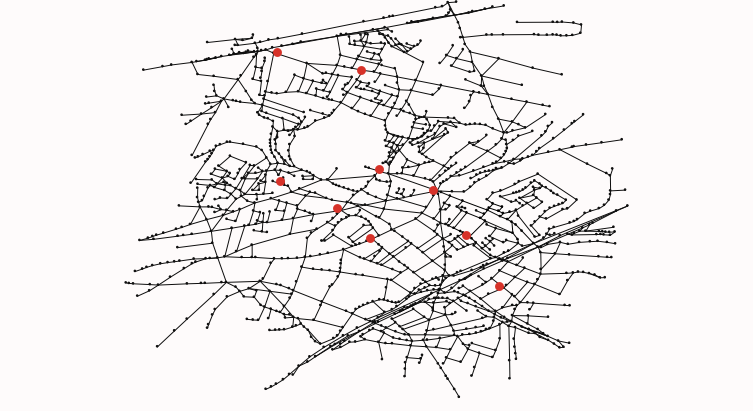
\includegraphics[width=0.45\textwidth]{Figures/NetworkGrowth/tick1}
%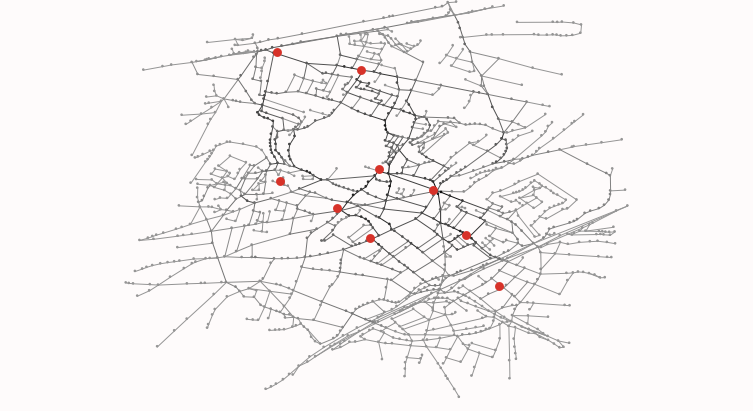
\includegraphics[width=0.45\textwidth]{Figures/NetworkGrowth/tick20}\\
%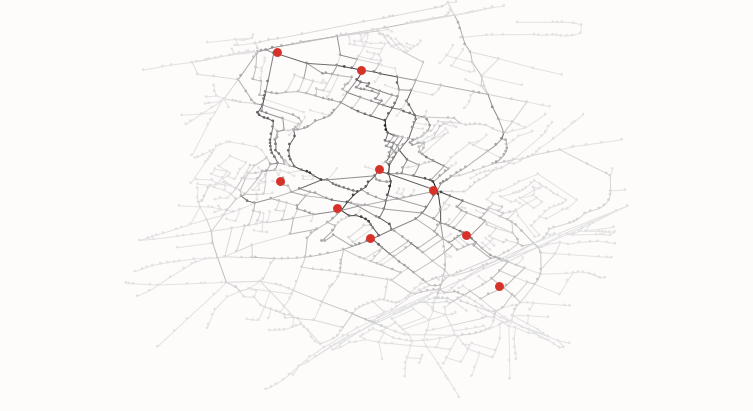
\includegraphics[width=0.45\textwidth]{Figures/NetworkGrowth/tick50}
%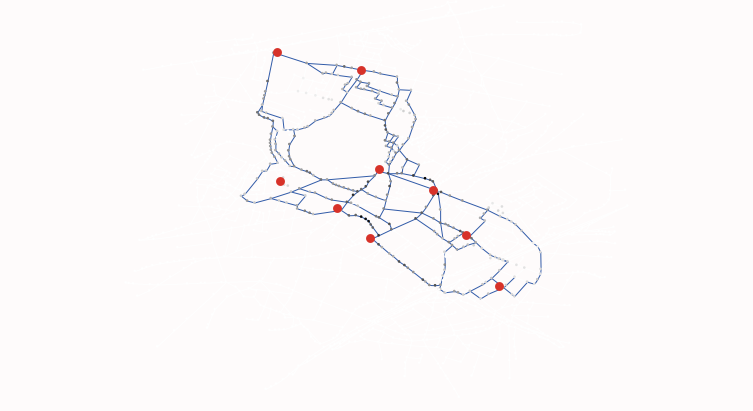
\includegraphics[width=0.45\textwidth]{Figures/NetworkGrowth/reseauFinal}
%\caption[Biological Network Growth][Croissance de réseau biologique]{Example of the application of the slime mould network generation model to the computation of an optimal public transportation network design.}{\comment{(Florent) source ?}}
%\label{fig:slimemould}
%\end{figure}
%%%%%%%%%%%%%%%%%%%%%%%

